\documentclass{article}
 
\usepackage{graphicx} 
\usepackage{amsmath}
\usepackage[para]{footmisc}
\usepackage{hyperref}
\usepackage{parskip}
\usepackage[utf8]{inputenc}
\usepackage[ngerman]{babel}
\usepackage[T1]{fontenc}

\usepackage{url}




\title{Abgabe 1 für Computergestützte Methoden}
\author{Gruppe (82), (Noel Michel (4342294), Moritz Bode (3859295), Paul Rinke (4337058)}
\date{1.12.2024}

\begin{document}

\maketitle
\tableofcontents

\newpage

\section{Der zentrale Grenzwertsatz}
Der zentrale Grenzwertsatz (ZGS) ist ein fundamentales Resultat der Wahr-
scheinlichkeitstheorie, das die Verteilung von Summen unabhängiger, identisch
verteilter (i.i.d.) Zufallsvariablen (ZV) beschreibt. Er besagt, dass unter 
bestimmten Voraussetzungen die Summe einer großen Anzahl solcher ZV annähernd
normalverteilt ist, unabhängig von der Verteilung der einzelnen ZV. Dies ist 
besonders nützlich, da die Normalverteilung gut untersucht und mathematisch
handhabbar ist.

\subsection{Aussage}
Sei $X1,X2,...,Xn$ eine Folge von $i.i.d.$ ZV mit dem Erwartungswert $\mu= E(Xi)$
und der Varianz $\sigma^2$ = $Var(Xi)$, wobei $0 < \sigma^2 < \infty$   gelte. Dann konvergiert die standardisierte Summe $Zn$ dieser ZV für $n\to\infty$ Verteilung gegen eine Standardnormalverteilung: $^1$
 
     
\begin{equation}
\label{eq:ZN}
 Zn=\frac{\sum_{i=1}^nXi-n\mu}{\sigma\sqrt{n}}\overset{d}{\longrightarrow} N(0,1).   
\end{equation}  

\noindent Das bedeutet, dass für große $n$ die Summe der ZV näherungsweise normalverteilt ist mit Erwartungswert $n\mu$ und $n\sigma^2$:

\begin{equation}
\label{Darstellung 2}
\sum_{i=1}^n Xi\sim N(n\mu,n\sigma^2).    
\end{equation}

 

\subsection{Erklärung der Standardisierung}

Um die Summe der $ZV$ in eine Standardnormalverteilung zu transformieren, subtrahiert man den Erwartungswert $n\mu$ und teilt durch die Standardnormalverteilung $\sigma\sqrt{n}$. Dies führt zu der obigen Formel \eqref{eq:ZN}. Die Darstellung \eqref{Darstellung 2} ist  für $n \to\infty$ nicht wohldefiniert. 

\subsection{Anwendungen}
Der ZGS wird in vielen Bereichen der Statistik und der Wahrscheinlichkeitstheorie angewendet. Typische Beispiele sind:

\begin{itemize}
    \item Berechnung von Konfidenzintervallen für Stichprobenmittelwerte
    \item Durchführung von Hypothesentests
\end{itemize}

\footnote{Der zentrale Grenzwertsatz hat verschiedene Verallgemeinerungen. Eine davon ist der \textbf{Lindeberg-Feller-Grenzwertsatz} \cite[Seite 328]{klenke}, der schwächere Bedingungen an die Unabhängigkeit und die identische Verteilung der ZV stellt.}

\newpage
\section{Bearbeitung zur Aufgabe 1}

\subsection{ Tabellenkalkulation}






\begin{figure}[ht]
    \centering
    \begin{minipage}{0.45\textwidth}
        \centering
        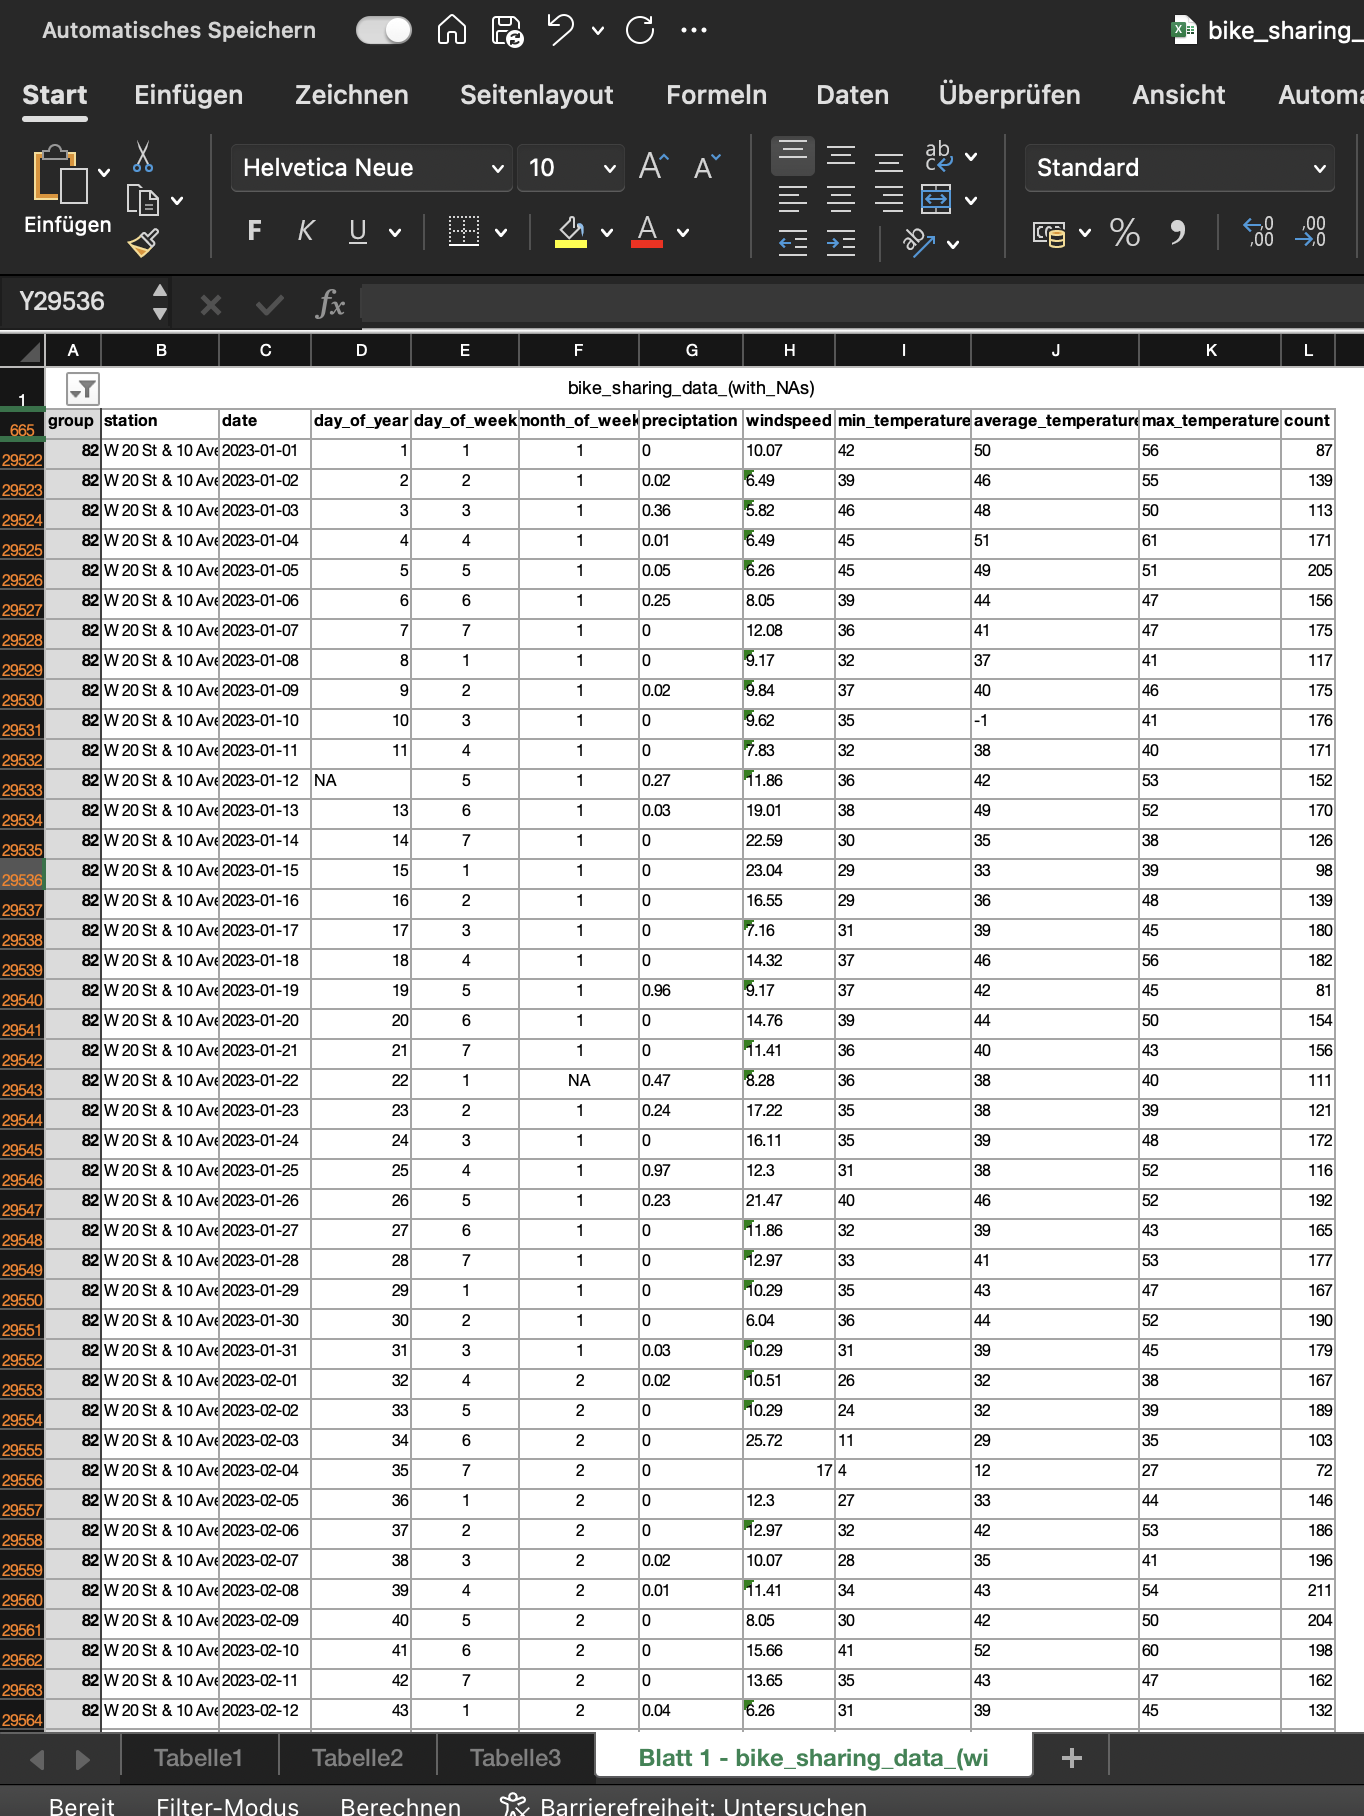
\includegraphics[width=\textwidth]{Tabellenkalkulation.png}
        \caption{Tabellenkalkulation}
        \label{fig:bild1}
    \end{minipage}
    \hfill
    \begin{minipage}{0.45\textwidth}
        \centering
        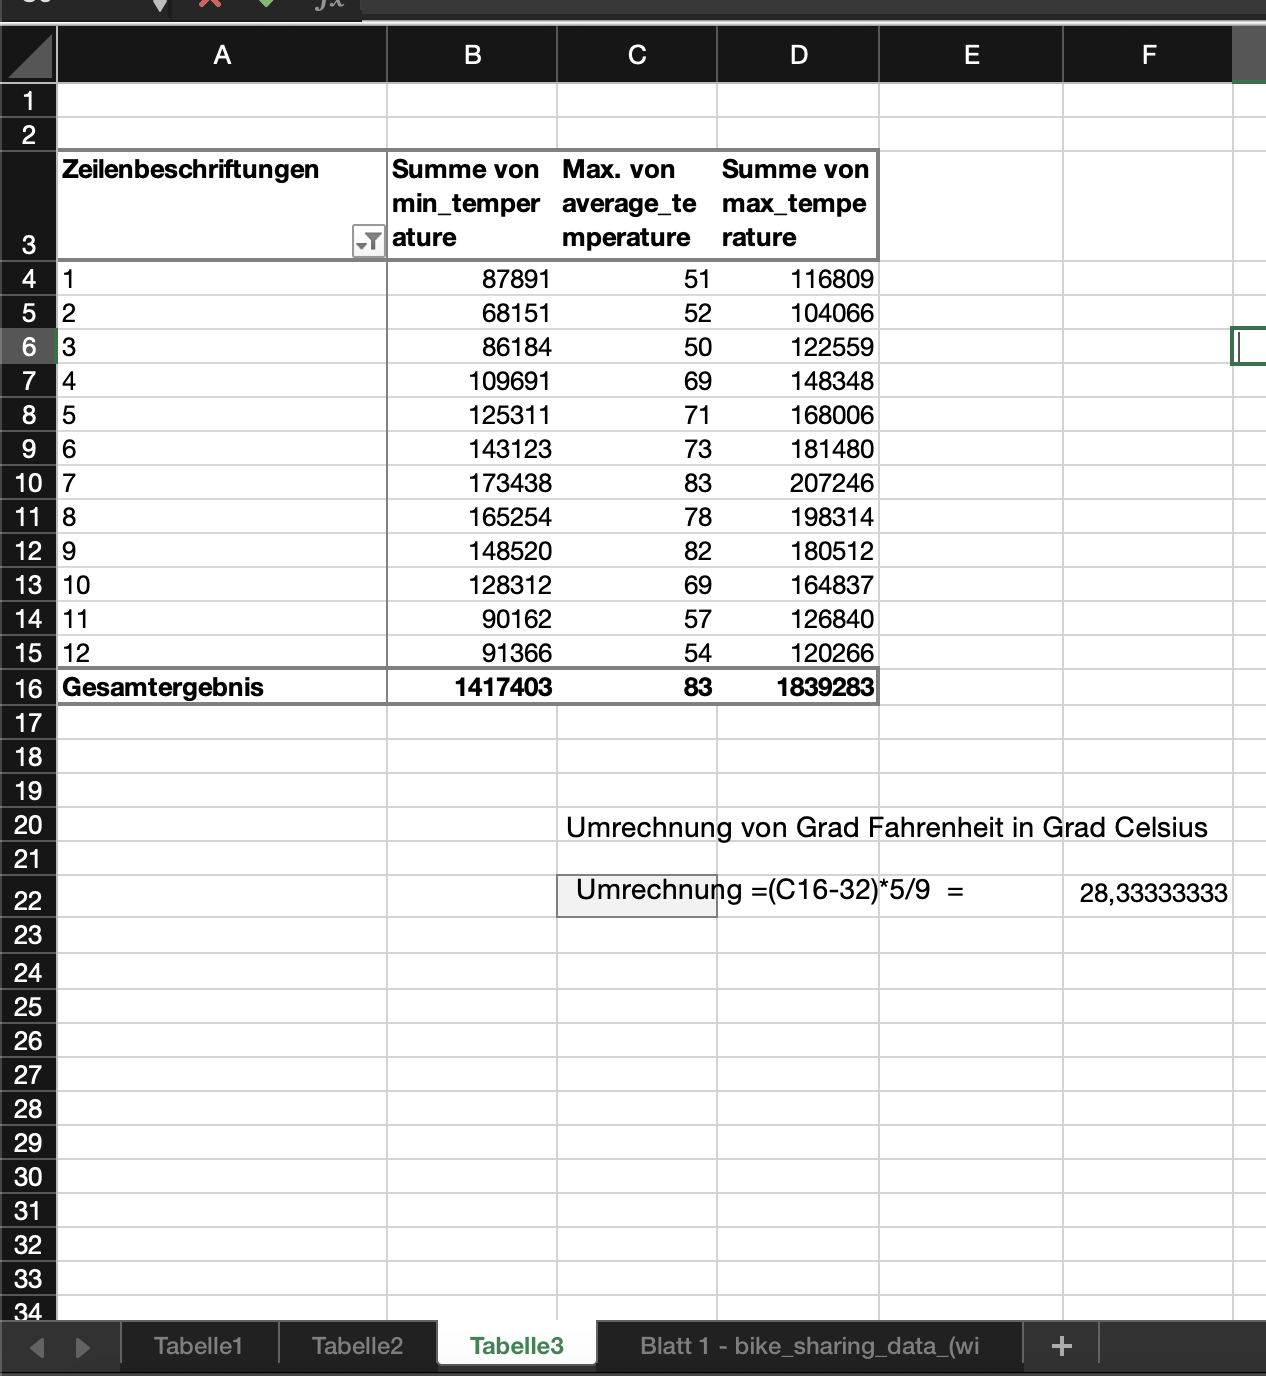
\includegraphics[width=\textwidth]{Pivot_Tabelle.png}
        \caption{Pivot Tabelle}
        \label{fig:bild2}
    \end{minipage}
   
\end{figure}




Um die höchste mittlere Temperatur zu berechnen haben wir zunächst die Daten in eine Tabellenkalkulation importiert. Daraufhin haben wir die die Daten für unsere Gruppe "82" relevanten Daten  gefiltert, sodass wir diese für diese eine Pivot Tabelle erstellen konnten. Für uns ist die Spalte Summe von average\_temperature relevant, durch Doppelklick auf die Zelle lässt sich auswählen, dass die Wertefelder nach maximalen Wert zusammengefasst werden sollen, wodurch als Gesamtergebnis die höchste mittlere Temperatur in Grad Fahrenheit angezeigt wird. Die Umrechnungsformel von Grad Fahrenheit in Grad Celsius lautet: $$Grad Celsius= (Grad Fahrenheit -32)*5/9$$ so kommen wir wie in Abbildung 2 zu entnehmen zu Ergebnis 28,33333333 Grad Celsius.

 
 \subsection{Datenbank-Schema entwerfen}

\textbf{1.Normalform}

Fahrradverleih(Team, StationID\# , Datum\#, Niederschlag,
Windgeschwindigkeit, niedrigste Temperatur, mittlere Temperatur, höchste Temperatur, Anzahl)

\textbf{2.Normalform}

Zeitrahmen(Datum\#, Tag des Jahres, Wochentag, Monat)

Stationen(StaionID\#, Name)


\subsection{Umsetzung des Schemas SQL}

\begin{verbatim}
    
PRAGMA foreign\_keys = ON;

CREATE TABLE stationen (
     StationID INTEGER PRIMARY KEY,
     Station TEXT NOT NULL
);
CREATE TABLE Zeitrahmen (
    Datum TEXT NOT NULL PRIMARY KEY,
    Tag\_des\_Jahres TEXT NOT NULL,
    Wochentag TEXT NOT NULL,
    Monat TEXT NOT NULL
);
CREATE TABLE Fahrradverleih(
    Team INTEGER,
    StationID INTEGER PRIMARY KEY,
    Datum TEXT NOT NULL PRIMARY KEY,
    Niederschlag INTEGER,
    Windgeschwindigkeit INTEGER,
    niedrigste\_Temperatur INTEGER,
    mittlere\_Temperatur INTEGER,
    höchste\_Temperatur INTEGER,
    Anzahl INTEGER,
FOREIGN KEY(StationID) REFERENCES Stationen(StationID)
FOREIGN KEY(Datum) REFERENCES Zeitrahmen(Datum)
);
\end{verbatim}

\subsection{Vorbereitung des Datensatzes}
Wir benennen in dem Ursprungsdatensatz die Namen der Spalten um in Team, Station , Datum, Tag des Jahres, Wochentag, Monat, Niederschlag,
Windgeschwindigkeit, niedrigste Temperatur, mittlere Temperatur, höchste Temperatur, Anzahl. In dem bearbeiteten Ursprungsdatensatz werden wir nun jeweils alle Zahlen der Spalten niedrigste Temperatur, mittlere Temperatur und höchste Temperatur in die Formel $(x-32)*(5/9)$ einsetzen und die Ergebnisse in den ursprünglichen Positionen ersetzen um Grad Fahrenheit in Grad Celsius zu ändern. Wir erstellen einen neuen Datensatz in Excel in dem wir eine Spalte mit dem Namen StationID erstellen und importieren die Spalte Station aus dem bearbeiteten Ursprungsdatensatz. In der Spalte StationID weisen wir nun jeder einzigartigen Station eine Nummer, in aufsteigender Folge, zu. Wir erstellen einen weiteren Datensatz in Excel und kopieren die Spalten Datum, Tag des Jahres, Wochentag und Monat in diesen.
Nun löschen wir aus dem bearbeiteten Ursprungsdatensatz die Spalten Tag des Jahres, Wochentag und Monat, und ersetzen die Spalte Station mit der Spalte StationID.

\subsection{SQL Abfrage für höchste mittlere Temperatur}
\begin{verbatim}
SELECT MAX(mittlere_Temperatur)
FROM Fahrradverleih
Where Team = 82
;
Ergebnis: 28,3
\end{verbatim}


\newpage

\bibliographystyle{plain}
\bibliography{references}
\end{document}
